\chapter{Codesigning Robots with Deep Reinforcement Learning}
\label{chp:contrib_CodesignRL}

This chapter will describe the process of designing the codesign loop, exploiting the theoretical foundation regarding deep reinforcement learning and evolutionary algorithms presented in \cref{chp:back_RLGA} and the conditioning of \ac{RBDA}s presented in \cref{chp:contrib_ABA} via a hardware accelerated physics simulator. In particular, each new individual created by the genetic algorithm will be evaluated by training a reinforcement learning agent with that set of parameters, for a predetermined task. The reward obtained will be interpreted as the fitness by the evolutionary algorithm, which will then select the best individuals and generate new ones, until the maximum number of generations is reached. In the first section, three reinforcement learning case studies will be presented, which will be used to test the framework. Then, the implementation details of the optimization based on the genetic algorithm will be discussed, together with an overview of the codesign loop. The resulting outcomes will be presented in \cref{chp:contrib_ResultsDiscussion}.


\section{Robot Codesign Framework}
\label{sec:Codesign}

The codesign loop starts in the evolutionary algorithm core, where the initial population is generated with a cardinality of $10$ individuals by sampling from a uniform distribution. Each individual is composed of a set of integers, each one representing an encoding of the motors available according to the \cref{tab:motorparams} as $\mathbf{0}: \text{Motor \textbf{XXXS}}, \mathbf{1}:\text{Motor \textbf{XXS}}, \dots, \mathbf{4}:\text{Motor \textbf{XXXL}}$. The initial population is then evaluated using the \ac{RL} framework, which runs in parallel with multiple agents having the same motor set and sharing the experience. Then, the sum of the rewards of the agents is associated with the fitness of that particular individual. Once the initial population has been evaluated, the evolutionary algorithm keeps the best individual in a process known as \textit{elitism} and mates the rest of the chromosomes. The mating process is performed using the \textit{one-point crossover} operator, which selects a random point in the chromosome and swaps the genes of the two parents. Then, the offspring is mutated using the \textit{uniform mutation} operator, which selects a random gene and mutates it with a probability of $0.2$. The process is then repeated for $20$ generations, after which the best individual is selected and its parameters are used to update the robot design, as represented in \cref{fig:codesignloop}.

\begin{figure}
    \centering
    \caption{Codesign Loop Flowchart.}
    \label{fig:codesignloop}
    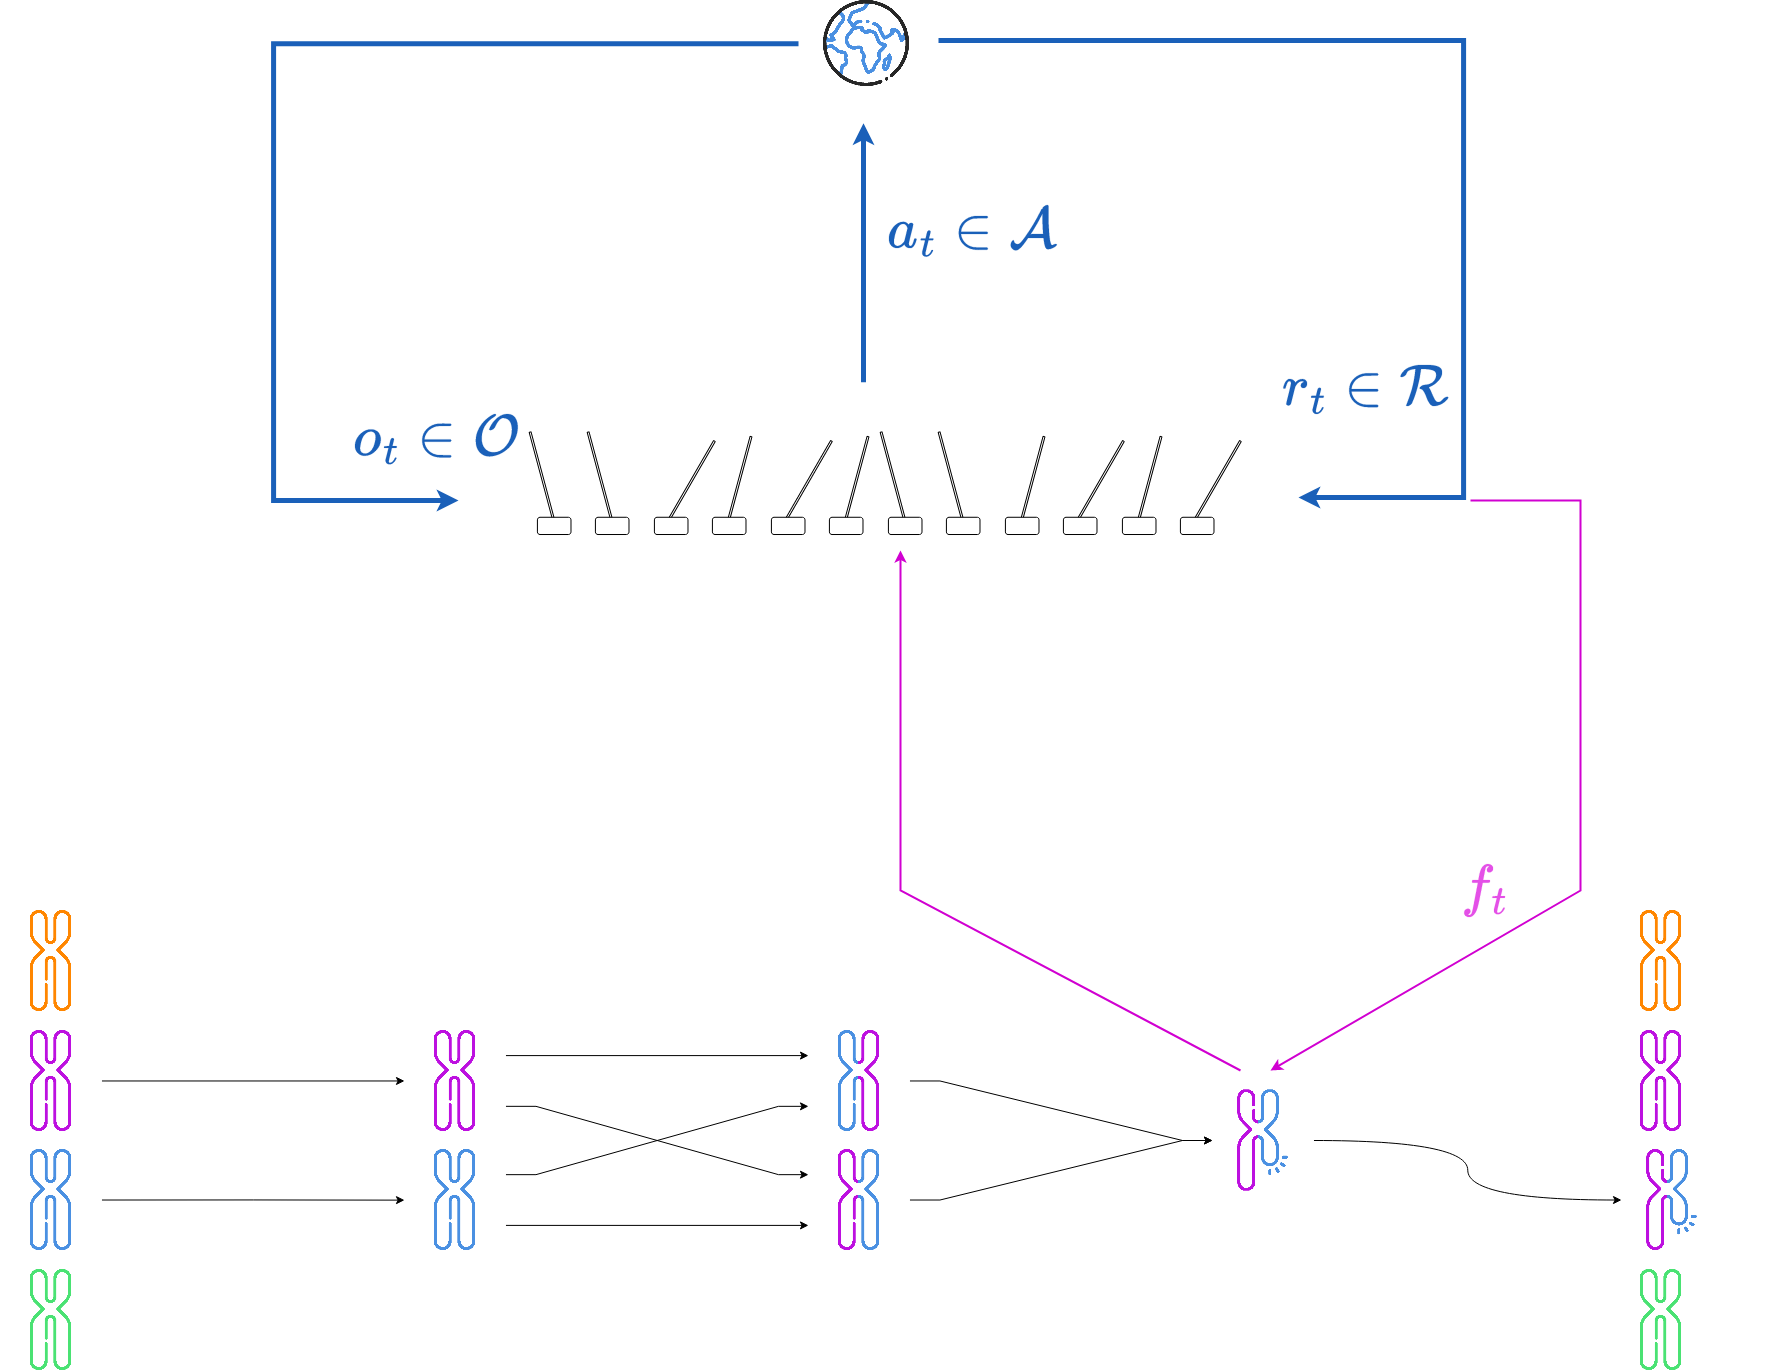
\includegraphics[width=.9\textwidth]{Images/codesign_loop.png}
\end{figure}

\section{Reinforcement Learning Case Studies}

In reinforcement learning scenarios, a crucial task is represented by the definition of the reward function, which is used to evaluate the performance of the agent. This process is usually called \textit{reward shaping}. The reward function is usually defined as a function of the state of the system, labeling it to be more or less desirable in order to achieve the intended behavior.

\subsection{Cartpole Swingup Task}

\begin{table}
    \centering
    \begin{tabular}{l c}
        \toprule
        \multicolumn{2}{c}{\textsc{Training Setup}} \\
        \midrule
        Model              & CartPole               \\
        Simulator          & JAXsim                 \\
        Simulation Device  & CPU                    \\
        Training Device    & GPU                    \\
        Training Framework & Stable Baselines 3     \\
        Used with Codesign & Yes                    \\
        \bottomrule
    \end{tabular}
    \caption{Cartpole Swingup Task -- Training Setup.}
\end{table}

\begin{figure}
    \centering
    \caption{JAXsim -- CartPole RL Training Visualization}
    \label{fig:cartpole}
    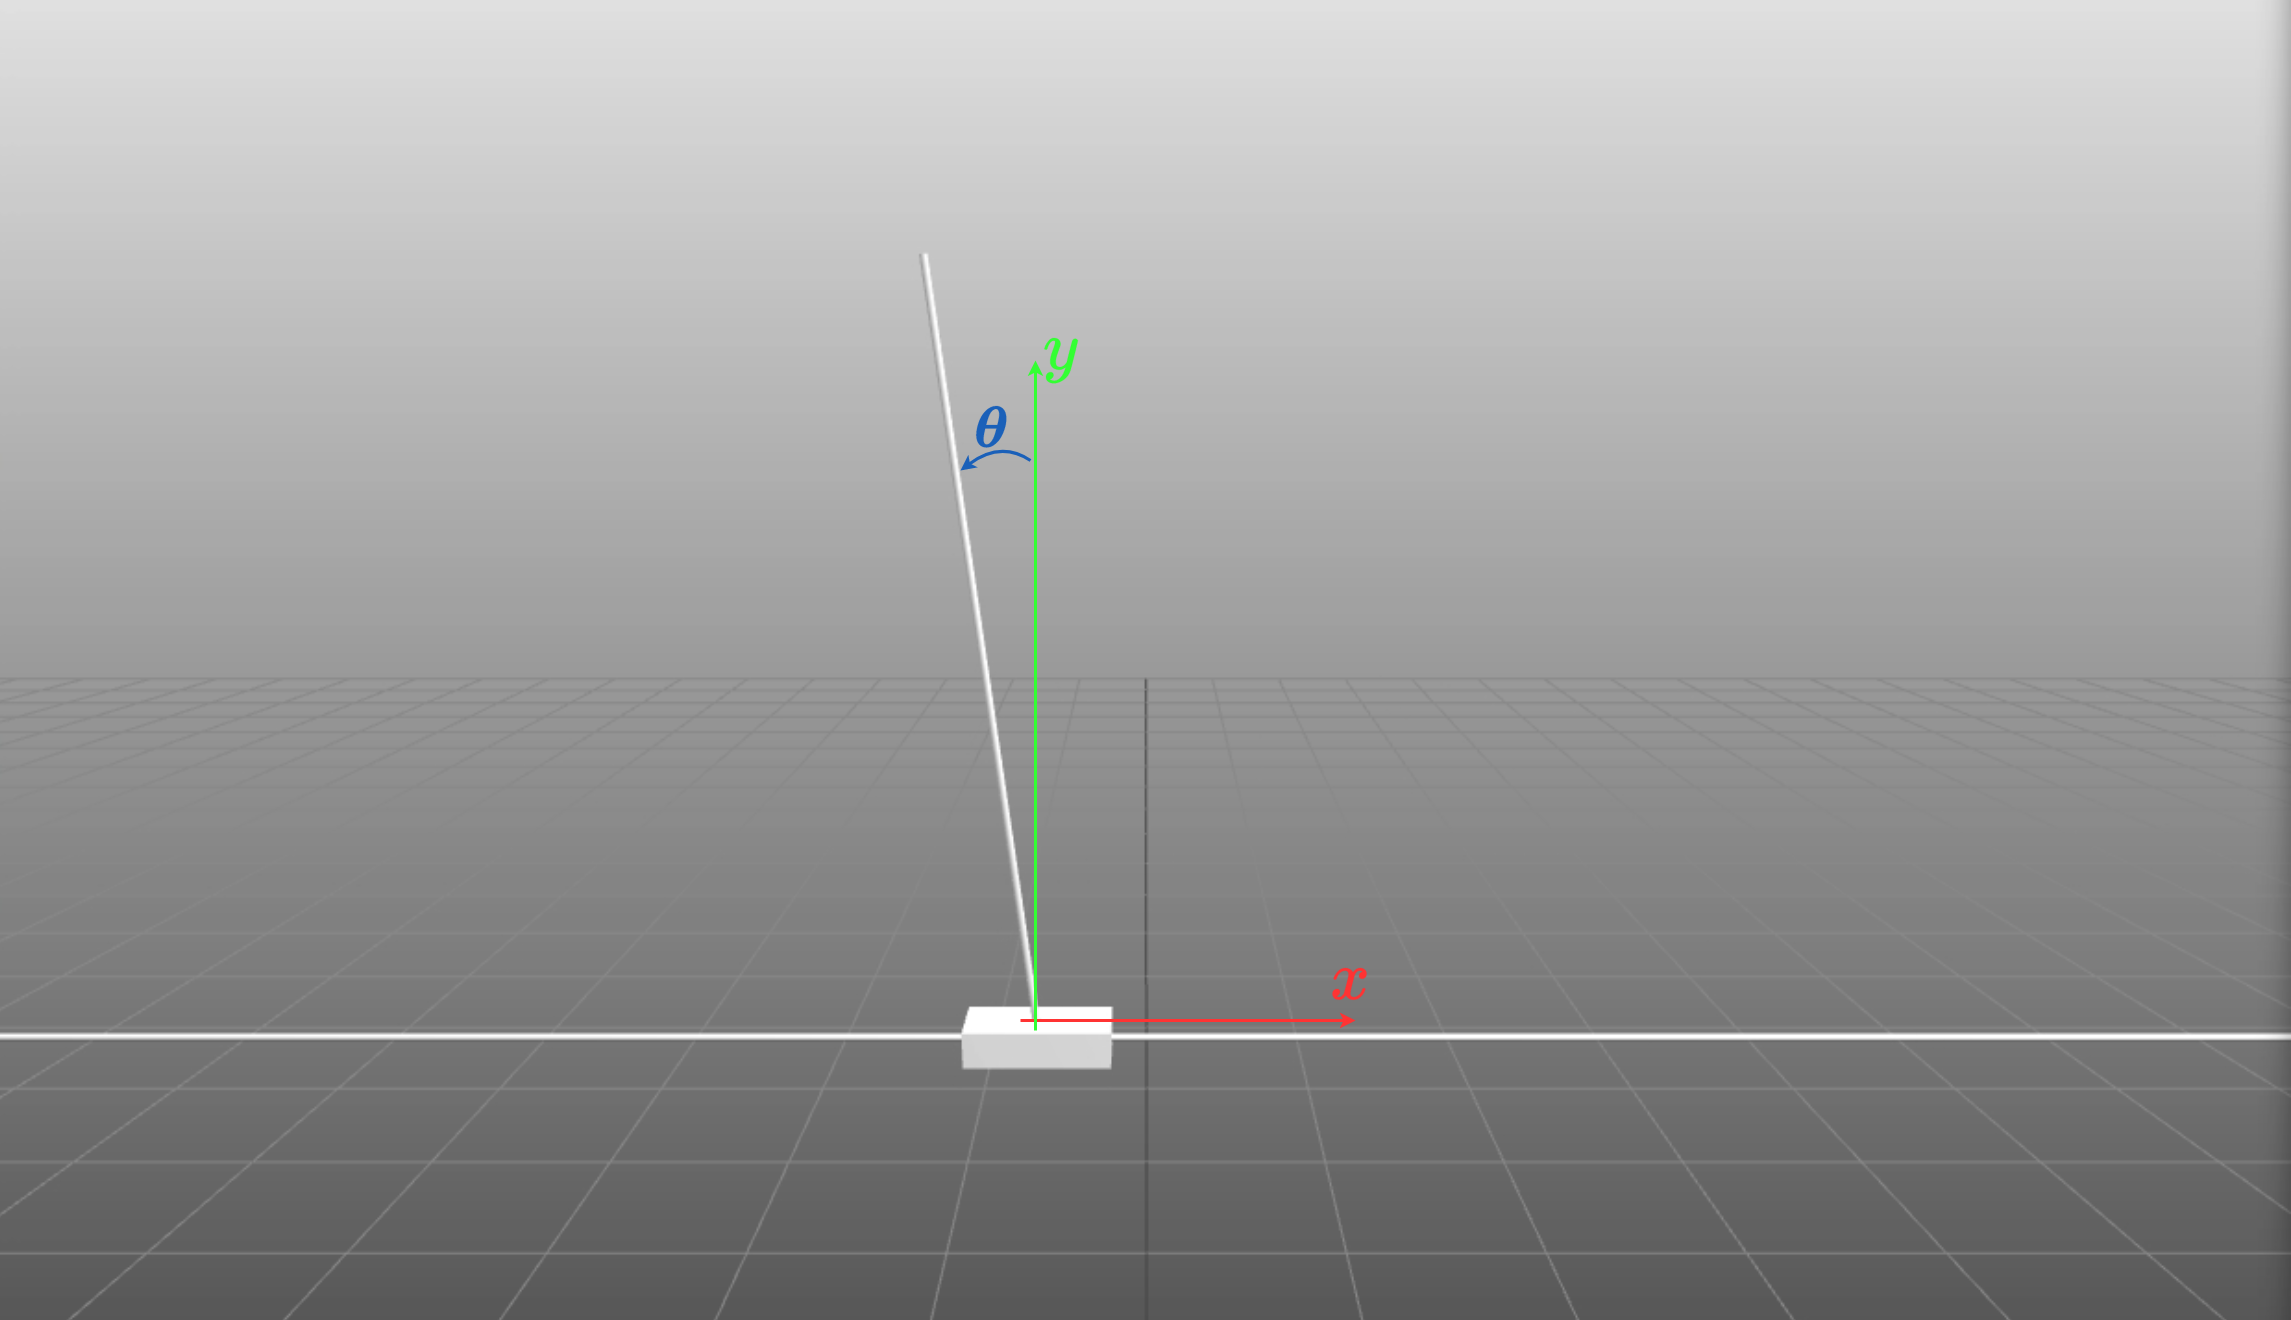
\includegraphics[width=0.7\textwidth]{Images/cartpole.png}
\end{figure}

The problem of codesign could easily become exponentially complex and computationally expensive, for this reason, the main focus of this work was to develop a scalable framework that could be customized in order to adapt to the complexity of the task as the computation resources increase in power. For this reason, the first task that has been used to test the \ac{RL} framework together with the \jaxsim simulator is the cartpole swingup task. In this task, the aim is to find a policy $\pi$ that is able to balance a pole attached to the cart, which is moving on a rail, and balance it to the upright position while minimizing the torques applied to the joints. In this case, the reward function is defined as a function of the state of the system, which is composed of the $x$-component of the position of the cart $x$, the velocity of the cart $\dot{x}$, the angle of the pole $\theta$ and the angular velocity of the pole $\dot{\theta}$:

\begin{equation}
    r _t = \begin{cases}
        n - \sum _i ^n \frac{\tau _i}{\tau _{\text{max}}} & \text{if } \left| \theta \right| < \theta_{\text{max}} \text{ and } \left| x \right| < x_{\text{max}} \\
        0                                                 & \text{otherwise}
    \end{cases}
\end{equation}

where $\theta_{\text{max}}$ and $x _{\text{max}}$ are respectively the imposed maximum angle of the pole from the vertical position and the maximum distance of the cart from the origin, $\tau _i$ is the torque applied to the $i$-th joint, $\tau _{\text{max}}$ is the maximum torque allowed and $n$ is the number of joints of the system.

\begin{figure}
    \centering
    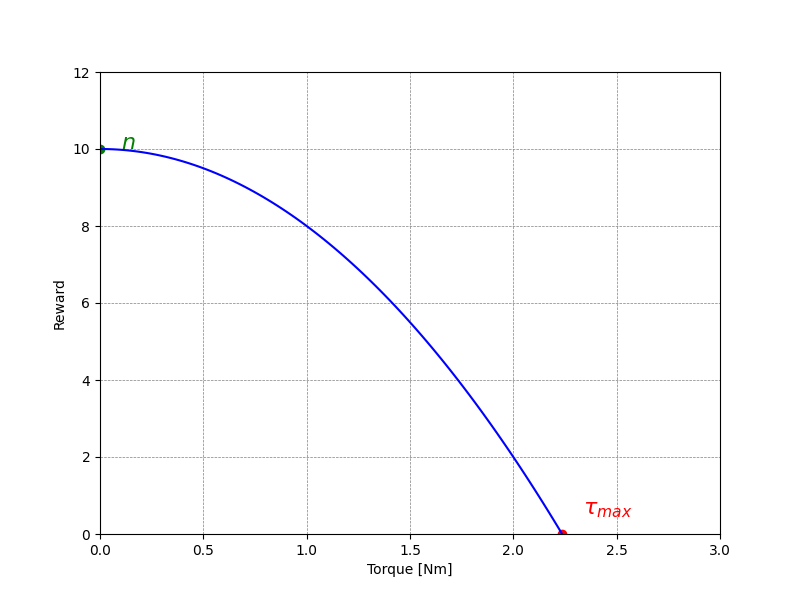
\includegraphics[width=0.8\textwidth]{Images/cartpole_reward.png}
    \caption{Cartpole Swingup Task -- Reward Function.}
    \label{fig:cartpolereward}
\end{figure}

The reward space is then defined to have a clear bound between positive and null reward, in order to make the learning process more stable the robot will have zero rewards when outside of the space defined by $\theta_{\text{max}}$ and $x _{\text{max}}$ and a reward that maximizes to the number of joints if the balance is achieved following a quadratic function dependent on the torques applied, as shown in \cref{fig:cartpolereward}. A penalty associated with the torques is also taken into account. It has a dual purpose, on the one hand, it allows minimizing the torques applied to the joints, on the other hand, it allows to effectively find an equilibrium position, which is not trivial in the case of a simple reward function based on the angle of the pole.

With that in mind, the action space will be defined as the set of torques applied to the joints, the observation space will be defined as the set of position and velocity of the cart and the pole, and the reward space will be a positive real number in the range $[0,2]$. The \cref{tab:cartpoleswinguptaskspacedef} summarizes the definition of the spaces used in this task.

\begin{table}
    \centering
    \label{tab:cartpoleswinguptaskspacedef}
    \begin{tabular}{l c}
        \toprule
        \textsc{Space}                  & \textsc{Projection Space} \\
        \midrule
        Action Space $\mathcal{A}$      & $\mathbb{R}$              \\
        Observation Space $\mathcal{S}$ & $\mathbb{R} ^{4}$         \\
        Reward Space $\mathcal{R}$      & $[0,1]$                   \\
        \bottomrule
    \end{tabular}
    \caption{Cartpole Swingup Task -- Space Definition.}
\end{table}

The trainings involving the cartpole swingup task and the codesign process have been performed on the \texttt{IITICUBWS065} machine whose specifications are reported in \cref{tab:rl_machine}.

\begin{table}[h]
    \centering
    \caption{\texttt{IITICUBWS065} Machine Specifications}
    \label{tab:rl_machine}
    \begin{tabular}[h]{l c}
        \toprule
        \textsc{Component}     & \textsc{Specification}                                                        \\
        \midrule
        \textbf{CPU}           & \begin{small}Intel(R) Xeon(R) Silver 4214 CPU @ 2.20GHz $\times 4$\end{small} \\
        \textbf{GPU}           & \begin{small}NVIDIA Quadro RTX 6000             \end{small}                   \\
        \textbf{RAM}           & \begin{small}384GB DDR4-3200                         \end{small}              \\
        \textbf{OS}            & \begin{small}Ubuntu 22.04.3 LTS                       \end{small}             \\
        \textbf{Kernel}        & \begin{small}5.15.0-88-generic        \end{small}                             \\
        \textbf{CUDA}          & \begin{small}12.2                                  \end{small}                \\
        \textbf{NVIDIA Driver} & \begin{small}535.129.03                             \end{small}               \\
        \bottomrule
    \end{tabular}
\end{table}

\subsection{Humanoid Locomotion Task}
The humanoid walking task is without a doubt one of the most challenging tasks in the field of robotics. The task aims to find a policy $\pi$ that is able to make the robot walk forward in a possibly \textit{human-like} motion. Its high complexity is mainly constituted by the necessity of controlling a large number of joints, which drastically increases the dimensionality of the problem, both in terms of action space and in observation space, from which it could be difficult to select the most relevant features for the algorithm.

All the \ac{RL} trainings for the humanoid walking task in this work have been performed on the \texttt{IITBMP014SRV001} machine whose specifications are reported in \cref{tab:srv001}.

\begin{table}[h]
    \centering
    \label{tab:srv001}
    \caption{\texttt{IITBMP014SRV001} Server Specifications}
    \begin{tabular}[h]{l c}
        \toprule
        \textsc{Component}     & \textsc{Specification}                                                       \\
        \midrule
        \textbf{CPU}           & \begin{small}AMD EPYC 7513 32-Core Processor @ 2.60GHz $\times 4$\end{small} \\
        \textbf{GPU}           & \begin{small}NVIDIA A100 80GB PCIe       $\times 2$             \end{small}  \\
        \textbf{RAM}           & \begin{small}1024GB DDR4-3200                         \end{small}            \\
        \textbf{OS}            & \begin{small}Ubuntu 22.04.3 LTS                       \end{small}            \\
        \textbf{Kernel}        & \begin{small}5.15.0-86-generic                        \end{small}            \\
        \textbf{CUDA}          & \begin{small}12.2                                  \end{small}               \\
        \textbf{NVIDIA Driver} & \begin{small}535.70.2                             \end{small}                \\
        \bottomrule
    \end{tabular}
\end{table}

\subsubsection{JAXsim Implementation}

\begin{table}
    \centering
    \begin{tabular}{l c}
        \toprule
        \multicolumn{2}{c}{\textsc{Training Setup}} \\
        \midrule
        Model              & ErgoCub                \\
        Simulator          & JAXsim                 \\
        Simulation Device  & CPU                    \\
        Training Device    & GPU                    \\
        Training Framework & Stable Baselines 3     \\
        Used with Codesign & No                     \\
        \bottomrule
    \end{tabular}
    \caption{ErgoCub Locomotion Task -- JAXsim Training Setup.}
\end{table}

\begin{figure}
    \centering
    \caption{JAXsim -- ErgoCub RL Training Visualization}
    \label{fig:ergocubtraining}
    \subfloat[ErgoCub Model \label{fig:ergocubmodel}]{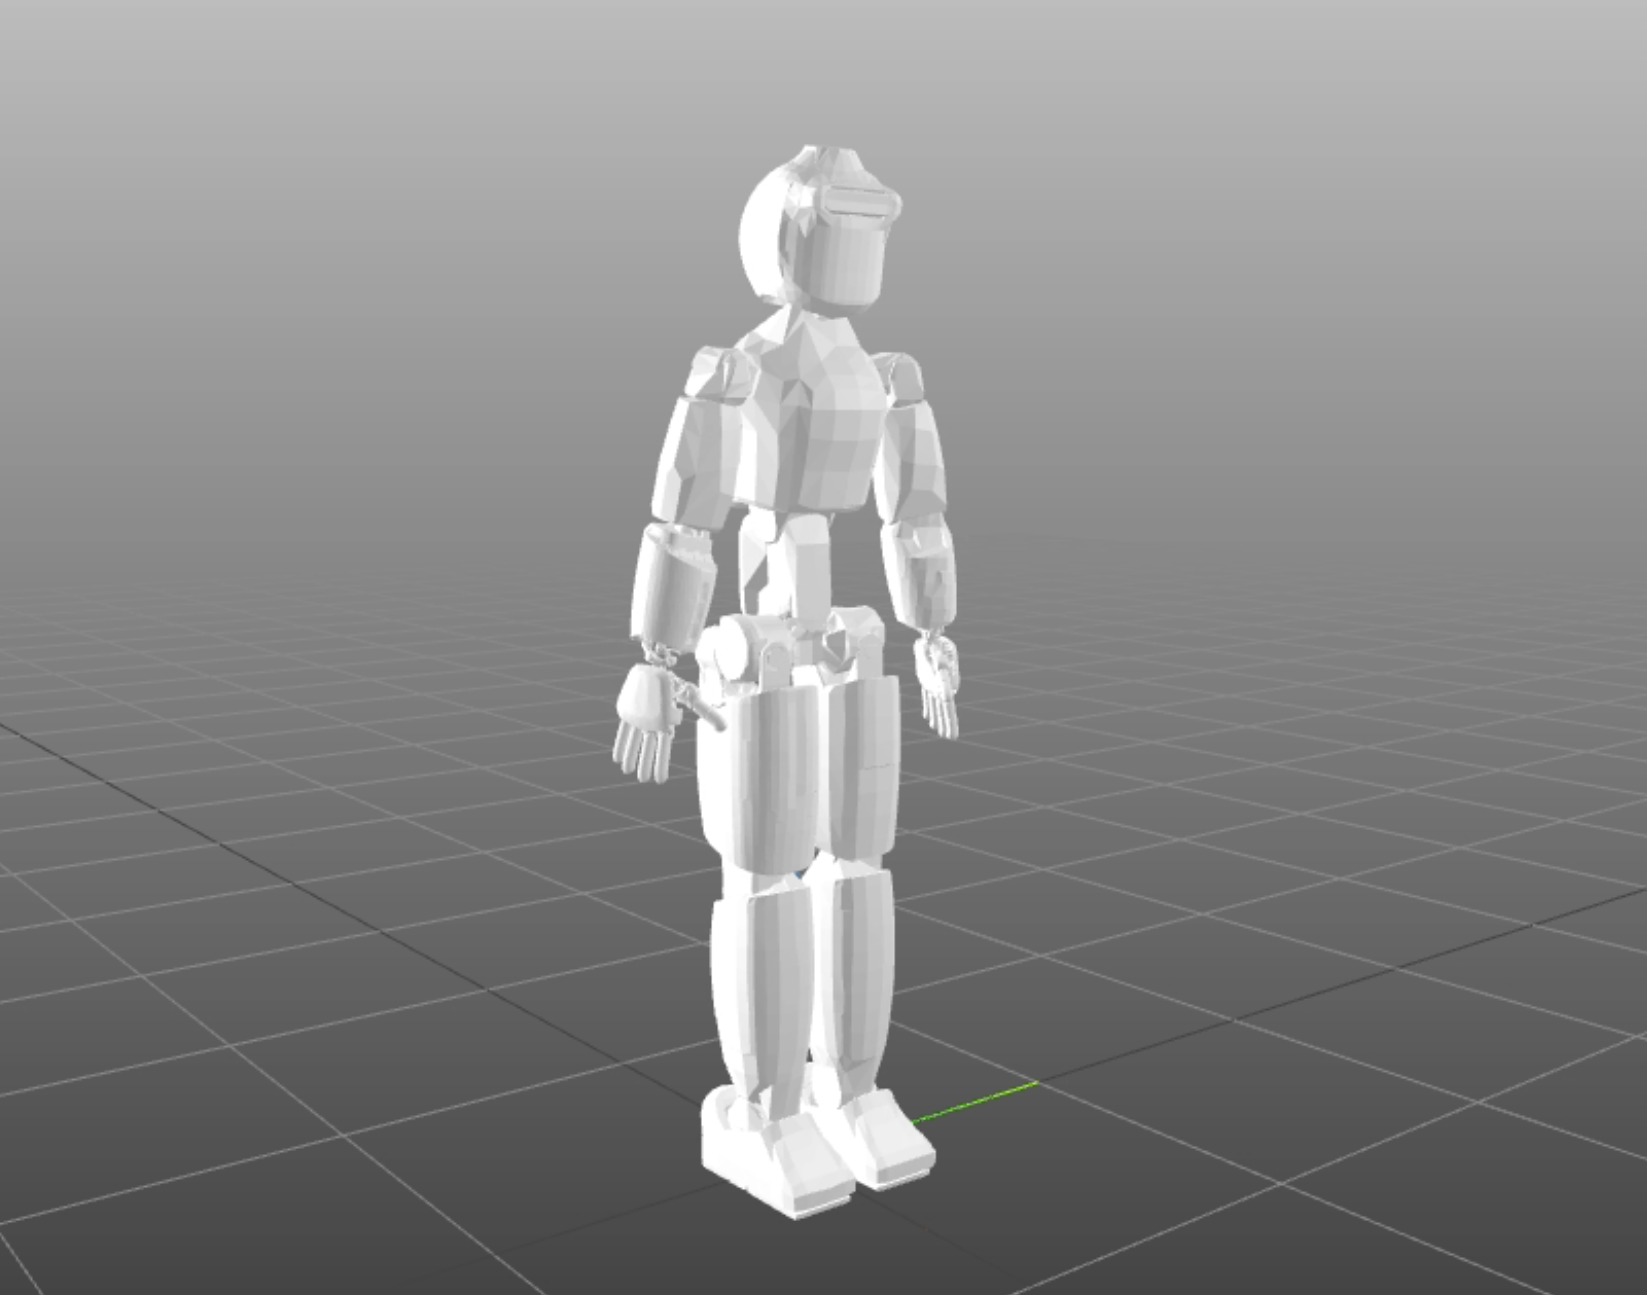
\includegraphics[width=.5\textwidth]{Images/ergocub_training.png}}
    \subfloat[ErgoCub Robot \label{fig:ergocub}]{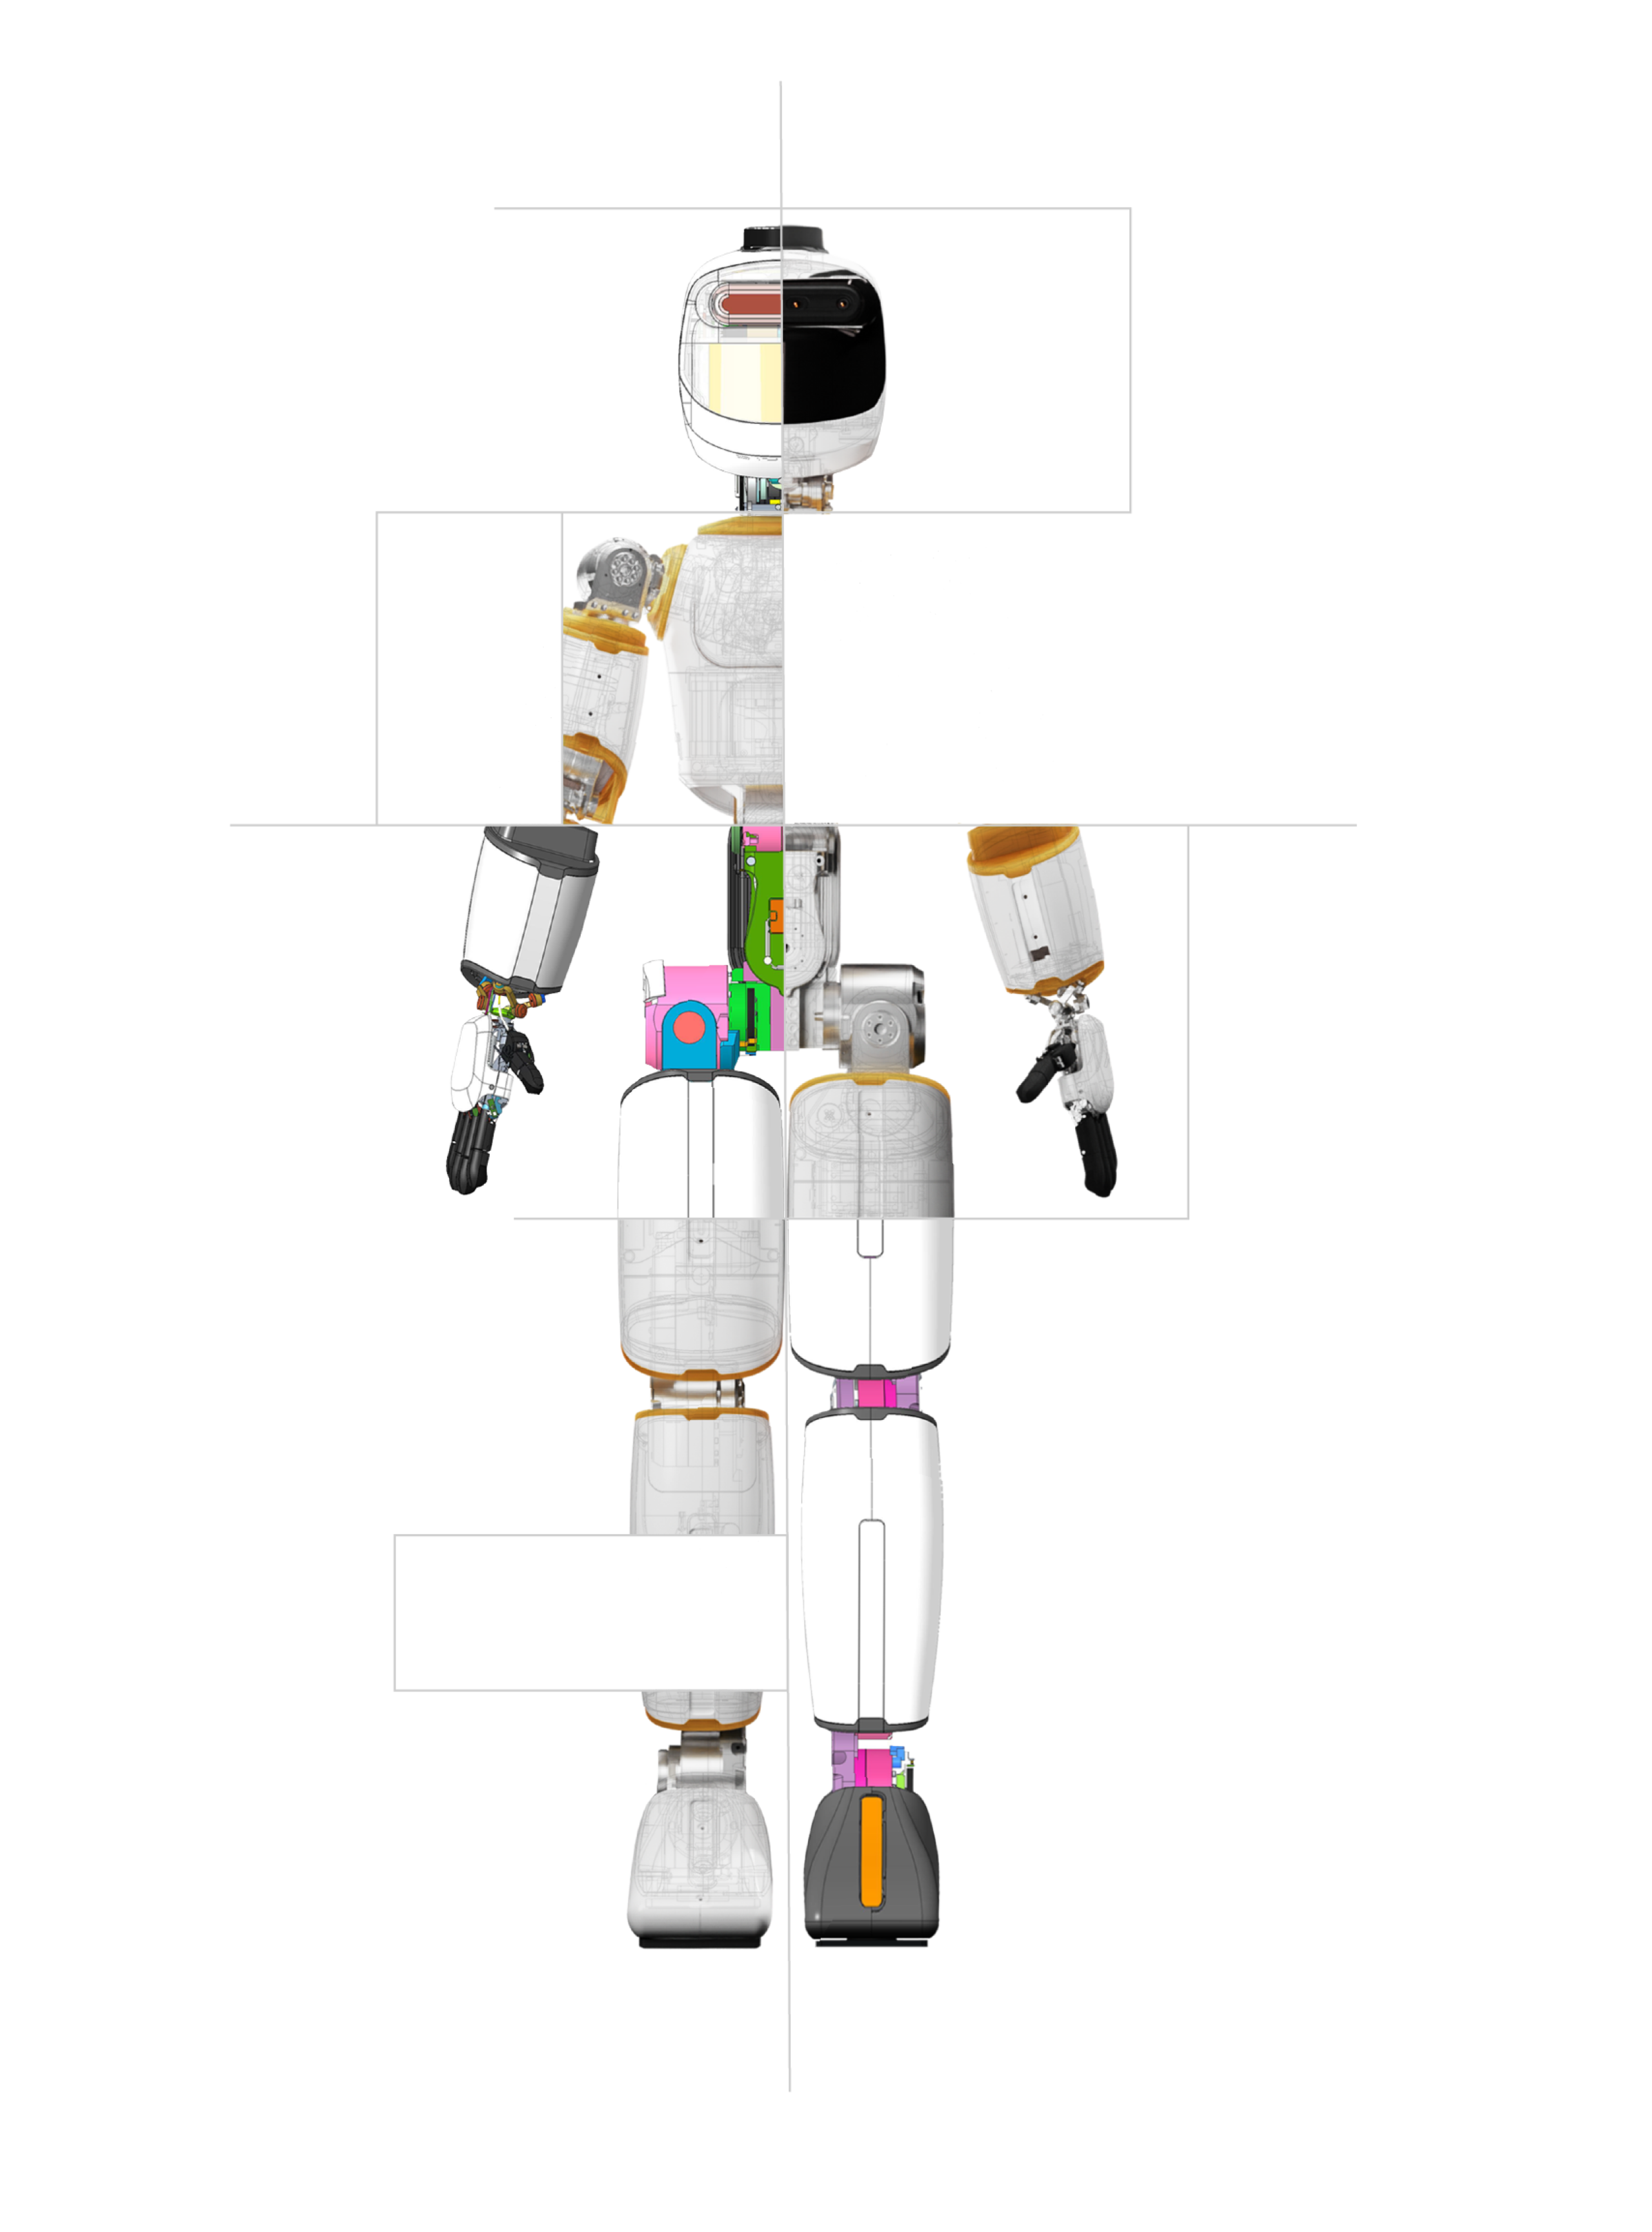
\includegraphics[width=.3\textwidth]{Images/ergocub.png}}
\end{figure}

The possibility to accelerate simulations using \ac{GPU}s on \jaxsim, makes it ideal in a reinforcement learning scenario. In fact, together with the possibility to precompile the Python code, it can speed up the training. The \ac{RL} framework has been implemented using the \texttt{Stable Baselines 3} library \citep{raffin_stable-baselines3_2021}, which supports the environment architecture by OpenAI Gym \citep{brockman_openai_2016}. In order to create an interface between the reinforcement learning baseline and \jaxsim, a custom class has been implemented so that at each agent step, the action is passed to the simulator, which then computes the next state and the reward, which are then returned to the agent.

At the aim of this task, the ErgoCub robot model, developed by the Italian Institute of Technology and shown in \cref{fig:ergocub}, has been used as the agent. The model \ac{URDF} file used reported in \cref{fig:ergocubmodel}, is an accurate representation of the real structure reported in \cref{fig:ergocub}, yet as not all the joints are relevant for the walking task, some of them were fixed and lumped together. The resulting model presents $6$ joints for each leg, $4$ for each arm and $3$ in the torso, for a total of $23$ joints actuated by $23$ motors.

\begin{equation}
    \label{eqn:ergocub_action_space}
    \mathcal{A} = \left\{ a \in \mathbb{R} ^{23} \mid -1 \leq a_i \leq 1 \right\}
\end{equation}

Hyperparameter tuning is a crucial part of the \ac{RL} framework, and it is often the most time-consuming part of the process. In this work, the hyperparameters were tuned using \texttt{optuna} \citep{akiba_optuna_2019}, a hyperparameter optimization framework, which uses \textit{Tree-structured Parzen Estimator} (\ac{TPE}) sampler with a median pruner, that models the objective function and suggests the next set of hyperparameters to evaluate. The hyperparameters tuned resulted in the values reported in \cref{tab:ppohyperparameters_jaxsim}.

\begin{table}[h]
    \centering
    \begin{tabular}{ll}
        \toprule
        \textsc{Parameter}          & \textsc{Value}          \\
        \midrule
        \multicolumn{2}{c}{\textbf{Training Parameters}}      \\
        Time Steps                  & $1e7$                   \\
        Batch size                  & $1,024$                 \\
        Number of Epochs            & $64$                    \\
        \midrule
        \multicolumn{2}{c}{\textbf{PPO Algorithm Parameters}} \\
        Clipping                    & $0.2$                   \\
        KL Target                   & $0.003$                 \\
        Discount Factor $\gamma$    & $0.99$                  \\
        GAE Parameter $\lambda$     & $0.9$                   \\
        SDE Sample Frequency        & $8$                     \\
        \midrule
        \multicolumn{2}{c}{\textbf{Coefficients}}             \\
        Value Function Coefficient  & $0.662$                 \\
        Entropy Coefficient $\beta$ & $0.0001$                \\
        \midrule
        \multicolumn{2}{c}{\textbf{Optimization Parameters}}  \\
        Learning Rate               & $0.0003$                \\
        Maximum Gradient Norm       & $0.8$                   \\
        \bottomrule
    \end{tabular}
    \caption{PPO Tuned Hyperparameters -- JAXsim Implementation}
    \label{tab:ppohyperparameters_jaxsim}
\end{table}

Given the high complexity of the problem, the network architecture composed of two separate networks, one for the policy and one for the value function, has been enlarged respect to the one used for the cartpole, in order to increase the capacity of the network to learn the task and to avoid the need of a large number of training iterations. In particular, the policy network is composed of two hidden layers of size $64$ and $64$ respectively, with a \ac{ReLU} activation function. The value function network is composed of three hidden layers of size $1024$, $512$, and $128$ respectively, with a \ac{ReLU} activation function, while the critic network has an architecture similar to the policy network, with the removal of the last hidden layer. The input of the policy network is then a vector of size $80$ composed of the observation space and the output is a vector of size $23$, equal to the action space size.
The output of the value network is a scalar, which is then used to compute the advantage function.

A tentative implementation has been performed using \textit{Long Short-Term Memory} (LSTM) neural networks, instead of simple \textit{Feed Forward} (FF) neural networks for the actor and the critic. \ac{LSTM} are a particular type of \textit{Recurrent Neural Networks} (RNNs) that, with the use of a \textit{forget gate}, are able to learn the temporal dependencies of the task avoiding the common issue of \ac{RNN}s of vanishing gradients. However, the results obtained with the \ac{LSTM} networks were not satisfactory, which is why the \ac{FF} networks have been used for the final implementation.

The final version of the implementation also featured an \textit{imitation learning} implementation starting from a bipedal locomotion configurations dataset. In this framework, the major weight of the reward was assigned to a $\ell_1$ loss between the robot pose and the target pose at each step, inducing the robot to be synchronized with the prior dataset samples. A \textit{Radial Basis Function} (\ac{RBF}) kernel was applied to the loss in order to make the reward function more robust to small errors in the pose, and the kernel width was then tuned for each component of the configuration, namely the position and the orientation of the root link and the joints positions, as reported in \cref{eqn:imitationlearning_jaxsim}:

\begin{equation}
    \label{eqn:imitationlearning_jaxsim}
    r _t = \sum _{\varepsilon \in \mathcal{E}} \gamma _{i _{prior}} e ^{-\gamma _{\epsilon} \varepsilon} - \gamma _{control} \sum _i ^{n} \tau _i ^2
\end{equation}

where $\gamma _{prior}$ and $\gamma _{control}$ are the weights of the prior and control terms, respectively, $\varepsilon$ is the error of the $j$-th term of the error function set $\mathcal{E}$ defined in \cref{eqn:err_function}, and $n$ is the number of degrees of freedom of the robot.

\begin{equation}[right=\empheqrbrace{}]
    \label{eqn:err_function}
    \mathcal{E} =
    \begin{cases}
        \varepsilon _{\text{orientation}}    := \lVert \mathbb{I}_3 - \mathbf{R}_{robot}^T \mathbf{R}_{prior}  \rVert _{\mathcal{F}}        \\
        \varepsilon _{\text{base position}}  := \lVert {}^w \mathbf{p}_B {} _{robot} - {}^w  \mathbf{p}_B {}_{prior}  \rVert _{\mathcal{F}} \\
        \varepsilon _{\text{joint positions}}:= \lVert s _{robot} - s _{prior}  \rVert _{\mathcal{F}}                                       \\
    \end{cases}
\end{equation}

where $\mathcal{F} \in \mathbb{R}$ is the Frobenius norm, $\mathbf{R}$ is an orientation represented as \textit{direction cosine matrix} of a unit quaternion, ${}^w \mathbf{p}_B$ is the base position $\in \mathbb{R} ^3$, $s$ is the vector of joint positions $\in \mathbb{R} ^{n}$, and $w$ is the world frame.
The orientation error $\mathcal{E} _{\text{orientation}} : \mathrm{SO}(3) \times \mathrm{SO}(3) \rightarrow [0, 2\sqrt{2}] \in \mathbb{R} ^+$ comes from \citep{huynh_metrics_2009}.

The \ac{RL} framework has been trained for $10^7$ steps, which given the episodic length, corresponds to $1024$ epochs. Thanks to the high number of available cores, the training took approximately $90$ minutes on the \texttt{IITBMP014SRV001} machine.

\begin{table}
    \centering
    \label{tab:walkingobs_jaxsim}
    \begin{tabular}{l c}
        \toprule
        \textsc{Observation} & \textsc{Dimension} \\
        \midrule
        Base Position        & $\mathbb{R} ^{3}$  \\
        Joints Positions     & $\mathbb{R} ^{23}$ \\
        Joints Velocities    & $\mathbb{R} ^{23}$ \\
        Actuation Torques    & $\mathbb{R} ^{23}$ \\
        Contact Points       & $\mathbb{R} ^{1}$  \\
        Target Position      & $\mathbb{R} ^{3}$  \\
        \bottomrule
    \end{tabular}
    \caption{JAXsim -- ErgoCub Locomotion Observation Space}
\end{table}

Throughout this project, the primary challenge in the Reinforcement Learning (\ac{RL}) framework was twofold. Firstly, the development of a contact model capable of accurately simulating the interaction between the robot and its environment. Simultaneously, it was crucial for this contact model to facilitate the algorithm's ability to forecast the agent's behavior, which could be difficult in the case of simple soft contact models as elucidated in \cref{sec:back_contacts}. Unfortunately, the \jaxsim simulator was in an early developmental stage for the walking task, i.e. for the contact model, which was not the central focus of this work. This made impossible to use the \jaxsim simulator for the humanoid walking task as the agent could not learn in an environment in which the contact dynamics was not predictable. Given the constraints of time available for thesis composition, we eventually opted to abandon this path and instead employed the more developed and readily available simulator, \textsc{Isaac Gym}, provided by NVIDIA.

\subsubsection{Isaac Gym Implementation}

\begin{table}
    \centering
    \begin{tabular}{l c}
        \toprule
        \multicolumn{2}{c}{\textsc{Training Setup}} \\
        \midrule
        Model              & ErgoCub                \\
        Simulator          & Isaac Gym              \\
        Simulation Device  & GPU                    \\
        Training Device    & GPU                    \\
        Training Framework & RL Games               \\
        Used with Codesign & No                     \\
        \bottomrule
    \end{tabular}
    \caption{ErgoCub Locomotion Task -- Isaac Gym Training Setup.}
\end{table}

\begin{figure}
    \centering
    \caption{Isaac Gym -- RL Training Visualization}
    \label{fig:isaacgymtraining}
    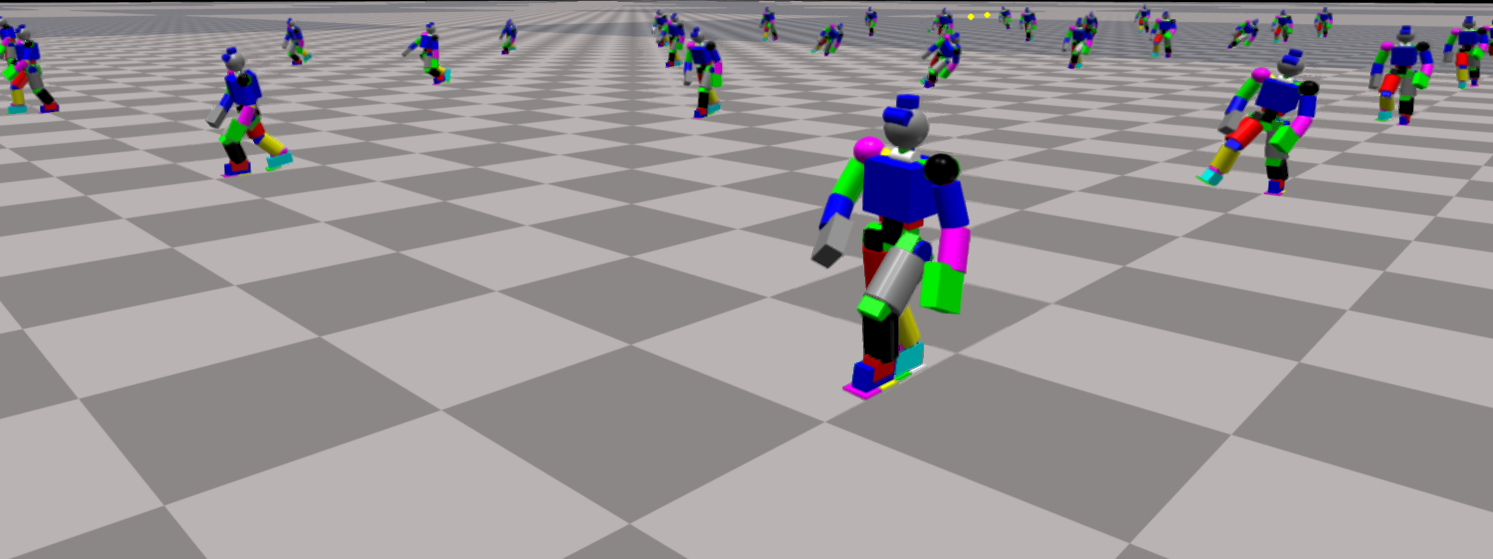
\includegraphics[width=.9\textwidth]{Images/stickbot_training_1.png}
\end{figure}

The humanoid walking task described in the following paragraphs has been achieved using \ac{PPO} together with the \ac{AMP} implementation from \texttt{rl\_games}. With this technique, there are two more networks involved to enhance the learning process and a dataset of trajectories that resembles the intended behaviour, in this case represented by a bipedal locomotion, is required. In this context, the AMP framework employs a generator network that creates data trying to imitate the prior and a discriminator network, whose task is to distinguish between the dummy trajectories generated and the actual samples from the prior dataset. The discriminator network is then used as a critic network to estimate the quality of the action taken.

As in the \jaxsim implementation, the ErgoCub model has been used, yet the meshes have been simplified to primitive shapes such as boxes, cylinders, and spheres, in order to reduce the computational cost of the simulation while maintaining the same dynamics of the original model. The observation space is then defined as per \cref{tab:walkingobs_isaacgym}, while the action space is formed as per \cref{eqn:ergocub_action_space}. With respect to the observation space defined in the \jaxsim implementation \cref{tab:walkingobs_jaxsim}, as this implementation uses \ac{AMP}, it is usually beneficial to include some reference frames position in the observation space, in order to allow the algorithm to learn the task faster.

\begin{table}
    \centering
    \label{tab:walkingobs_isaacgym}
    \begin{tabular}{l c}
        \toprule
        \textsc{Observation}  & \textsc{Dimension}         \\
        \midrule
        Root Link Height      & $\mathbb{R}$               \\
        Root Link Orientation & $\mathbb{R} ^{4}$          \\
        Root Link Velocity    & $\mathbb{R} ^{6}$          \\
        Joints Positions      & $\mathbb{R} ^{23}$         \\
        Joints Velocities     & $\mathbb{R} ^{23}$         \\
        Key Frames Position   & $\mathbb{R} ^{4 \times 6}$ \\
        \bottomrule
    \end{tabular}
    \caption{Isaac Gym -- Humanoid Locomotion Observation Space.}
\end{table}

Rewards, actions, and observations are then normalized to the range $[0,1]$ in order to make the learning process more stable and to avoid the need to tune the reward function for different robots. The \cref{tab:cartpoletaskspacedef} summarizes the definition of the spaces used in the \ac{RL} framework.

\begin{table}
    \centering
    \caption{Humanoid Walking Task -- Space Definition.}
    \label{tab:cartpoletaskspacedef}
    \begin{tabular}{l c}
        \toprule
        \textsc{Space}                  & \textsc{Projection Space} \\
        \midrule
        Action Space $\mathcal{A}$      & $\mathbb{R} ^{23}$        \\
        Observation Space $\mathcal{S}$ & $\mathbb{R} ^{75}$        \\
        Reward Space $\mathcal{R}$      & $[0,1]$                   \\
        \bottomrule
    \end{tabular}
\end{table}


\section{Evolutionary Algorithm Core}
\label{sec:EvolutionAlgo}

The evolutionary algorithm has been used in the codesign loop to select three main motor parameters from a discrete search space. The evolutionary algorithm has been based on the \texttt{deap} library \citep{DEAP_JMLR2012}.

The motor set of parameters is composed of three main components: motor inertia $\mathbb{M}^M$, motor viscous friction $\mathbf{K}_v$, and gear ratio $\boldsymbol{\Gamma}$. At each iteration, the fitness is computed using the \ac{RL} framework, which returns the reward associated with the individual. The reward is then used as the fitness function of the evolutionary algorithm. The evolutionary algorithm then selects the best individuals, which are then used to update the population. The process is then repeated until it reaches the maximum number of generations. The total number of combination are given by the following equation:

\begin{equation}
    H = n^k = 2^9 = 512
\end{equation}

where $n$ is the number of joints and $k$ is the number of motors.

The evolutionary algorithm has been used to select the motor parameters from the set of possible values. The discrete set of possible values for each parameter shown in the \cref{tab:motorparams} has been based on a set of motors used in the ErgoCub robot.

\begin{table}[h]
    \centering
    \begin{tabular}{c c c c}
        \toprule
        \textsc{Motor} & \textsc{Inertia} $[k\mathrm{gm}^2]$ & \textsc{Gear Ratio} & \textsc{Viscous Friction} $[\mathrm{N}s\mathrm{rad}^{-1}]$ \\
        \midrule
        \textbf{XXXS}  & $0.0001$                            & $1/100.0$           & $0.05$                                                     \\
        \textbf{XXS}   & $0.0001$                            & $1/100.0$           & $0.075$                                                    \\
        \textbf{XS}    & $0.0001$                            & $1/100.0$           & $0.1$                                                      \\
        \textbf{S}     & $0.0001$                            & $1/100.0$           & $0.1$                                                      \\
        \textbf{M}     & $0.001$                             & $1/100.0$           & $0.15$                                                     \\
        \textbf{L}     & $0.001$                             & $1/160.0$           & $0.2$                                                      \\
        \textbf{XL}    & $0.001$                             & $1/160.0$           & $0.25$                                                     \\
        \textbf{XXL}   & $0.001$                             & $1/160.0$           & $0.3$                                                      \\
        \textbf{XXXL}  & $0.001$                             & $1/160.0$           & $0.35$                                                     \\
        \bottomrule
    \end{tabular}
    \caption{Motor Set Parameters.}
    \label{tab:motorparams}
\end{table}


Considering the computation-expensive nature of the \ac{RL} framework, the hyperparameters for the evolutionary algorithm have been tuned to prefer a more explorative approach, in order to avoid the need for a large number of generations. In particular, the following hyperparameters have been selected:

\begin{table}
    \centering
    \begin{tabular}{ll}
        \toprule
        \textsc{Parameter}    & \textsc{Value} \\
        \midrule
        Population Size       & $10$           \\
        Number of Generations & $20$           \\
        Crossover Probability & $0.5$          \\
        Mutation Probability  & $0.2$          \\
        \bottomrule
    \end{tabular}
    \caption{Evolutionary Algorithm Hyperparameters.}
\end{table}
